\documentclass{beamer}

\usepackage[T2A]{fontenc}
\usepackage[utf8]{inputenc}
\usepackage{amssymb,amsfonts,amsmath}
\usepackage{proof}
\usepackage{graphicx}
\graphicspath{{img/}}
\usepackage[english,russian]{babel}
\usetheme{Boadilla}
\title[Типизированный интерпретатор $\lambda_\rightarrow$]{Типизированный интерпретатор $\lambda$-исчисления \\ Повышаем уверенность в корректности с помощью типов}
\author{Артём Шалхаков}
\institute{ТЭАКТ}
\date{28-е июня 2010}

\begin{document}
\frame{\titlepage}
\frame{\tableofcontents}

\section{Введение}
\subsection{Мотивация}

\frame{
  \frametitle{Зачем и почему?}
  \begin{itemize}
    \item Языки и интерпретация играют ключевую роль в информатике
    \item Важно знать, что интерпретатор подчиняется спецификации
  \end{itemize}
}
\frame{
  \frametitle{Ошибки в программах}
  \begin{itemize}
    \item Увы, распространённое явление
    \item Нужно что-то с этим делать
      \begin{itemize}
        \item Мы улучшаем инструменты
      \end{itemize}
  \end{itemize}
}

\subsection{Работы в области}
\frame{
  \frametitle{Множество подходов}
  \begin{itemize}
    \item Тестирование
      \begin{itemize}
        \item TDD
        \item unit-тесты
        \item Начни с тестов
      \end{itemize}
    \item (Формальная) верификация
      \begin{itemize}
        \item Автоматизированные инструменты
           \begin{itemize}
             \item Coq, Isabelle, HOL
             \item Z, Alloy
           \end{itemize}
        \item К истине через доказательство
        \item \emph{Очень} тяжеловесно
      \end{itemize}
  \end{itemize}
}
\frame{
  \frametitle{Современные типизированные ФЯП}
  \begin{itemize}
     \item Haskell, OCaml, SML, ATS
     \item Проверка типов постепенно приближается к автоматизированному доказательству теорем
     \item Типы как формулы, программы как доказательства
     \item Легковесная верификация
  \end{itemize}
}
\frame{
  \frametitle{Теоретическая база 1}
  \begin{itemize}
    \item Натуральная дедукция для логики высказываний
   \item Синтаксис: $A$ ::= $x \in V$ | $A_1 \land A_2$ | $A_1 \lor A_2$ | $A_1 \implies A_2$ | $A_1 \iff A_2$ | $\bot$ | $\neg A$
   \item Контекст: $\Gamma$ ::= $\emptyset$ | $\Gamma, A$ | $\Gamma_1, \Gamma_2$
   \item Правила вывода:
     \begin{enumerate}
       \item $$\infer[(axiom)]{A \vdash A}{}$$
       \item $$\infer[(abst)]{\Gamma \vdash B \implies A}{\Gamma, B \vdash A}$$
       \item $$\infer[(app)]{\Gamma \vdash A}{\Gamma \vdash B \implies A & \Gamma \vdash B}$$
     \end{enumerate}
  \end{itemize}
}
\frame{
  \frametitle{Теоретическая база 2}
  \begin{itemize}
    \item Бестиповое $\lambda$-исчисление
    \item Синтаксис: $e$ ::= $x \in V$ | $\lambda x. e$ | $e_1 e_2$
    \item Правила переписывания:
    \begin{enumerate}
\item $\alpha$-конверсия (переименование): $\lambda x_i.e \Leftrightarrow \lambda x_j.[x_j/x_i]e$, где $x_j \notin fv(e)$
\item $\beta$-конверсия (подстановка): $(\lambda x.e_1)e_2 \Leftrightarrow [e_2/x]e_1$
\item $\eta$-конверсия: $\lambda x.(e x) \Leftrightarrow e$, если $x \notin fv(e)$
    \end{enumerate}
  \end{itemize}
}
\frame{
  \frametitle{Теоретическая база 3}
  \begin{itemize}
    \item Простое типизированное $\lambda$-исчисление
    \item Синтаксис:
\begin{itemize}
\item Термы $e$ ::= $x \in V$ | $\lambda x : \tau. e$ | $e_1 e_2$ | $n$ \\
\item Значения $v$ ::= $\lambda x : \tau. e$ | $n$ \\
\item Типы $\tau$ ::= int | $\tau_1 \implies \tau_2$
\end{itemize}
    \item Контекст $\Gamma$ ::= $\emptyset$ | $\Gamma, x:\tau$
    \item Отношение типизации
$$\infer[(var)]{\Gamma \vdash x:\tau}{\Gamma (x) = \tau}$$
$$\infer[(int)]{\Gamma \vdash n:int}{}$$
$$\infer[(abst)]
  {\Gamma \vdash \lambda x:\tau_1 . e : \tau_1 \implies \tau_2}
  {\Gamma,x:\tau_1 \vdash e:\tau_2}
$$
$$\infer[(app)]
  {\Gamma \vdash e_1 e_2 : \tau_2}
  {\Gamma \vdash e_1:\tau_1 \implies \tau_2 & \Gamma \vdash e_2:\tau_1}
$$
  \end{itemize}
}

\section{Наш вклад}
\subsection{Подход}
\frame{
  \frametitle{Типизированное внутреннее представление}
  \begin{itemize}
    \item Типы \emph{объектного} языка отражаются в типах \emph{мета}-языка
    \item Возможно благодаря выразительной системе типов ATS
  \end{itemize}
}

\subsection{Достоинства и недостатки}
\frame{
  \frametitle{Основные моменты}
  \begin{itemize}
    \item Проверка типов (нетипизированное $\rightarrow$ типизированное представление)
    \item Типобезопасный вычислитель
    \item Расширения для просто-типизированного $\lambda$-исчисления
      \begin{itemize}
        \item Общая рекурсия (полнота по Тьюрингу)
        \item Числа и булевы переменные
        \item Пары и объединения
        \item Конструкции \emph{if}, \emph{case}
      \end{itemize}
    \item Возможные расширения
      \begin{itemize}
        \item Ввод-вывод
        \item Определяемые пользователем типы данных
        \item Изменяемые структуры данных
        \item Параметрический полиморфизм
      \end{itemize}
  \end{itemize}
}
\frame{
  \frametitle{Ограничения}
  Не все возможные инварианты проверяются
  \begin{itemize}
    \item Связывание переменных и подстановка
    \item Завершимость
    \item От правил редукции до SECD-машины
  \end{itemize}
  Но этого достаточно для практических целей.
}

\section{Заключение}
\frame{
  \frametitle{Результаты}
  \begin{itemize}
    \item Проверка типов и вычислитель
    \item Оно работает!
  \end{itemize}
}
\frame{
  \begin{figure}
    % [width=0.75\linewidth]
    \center{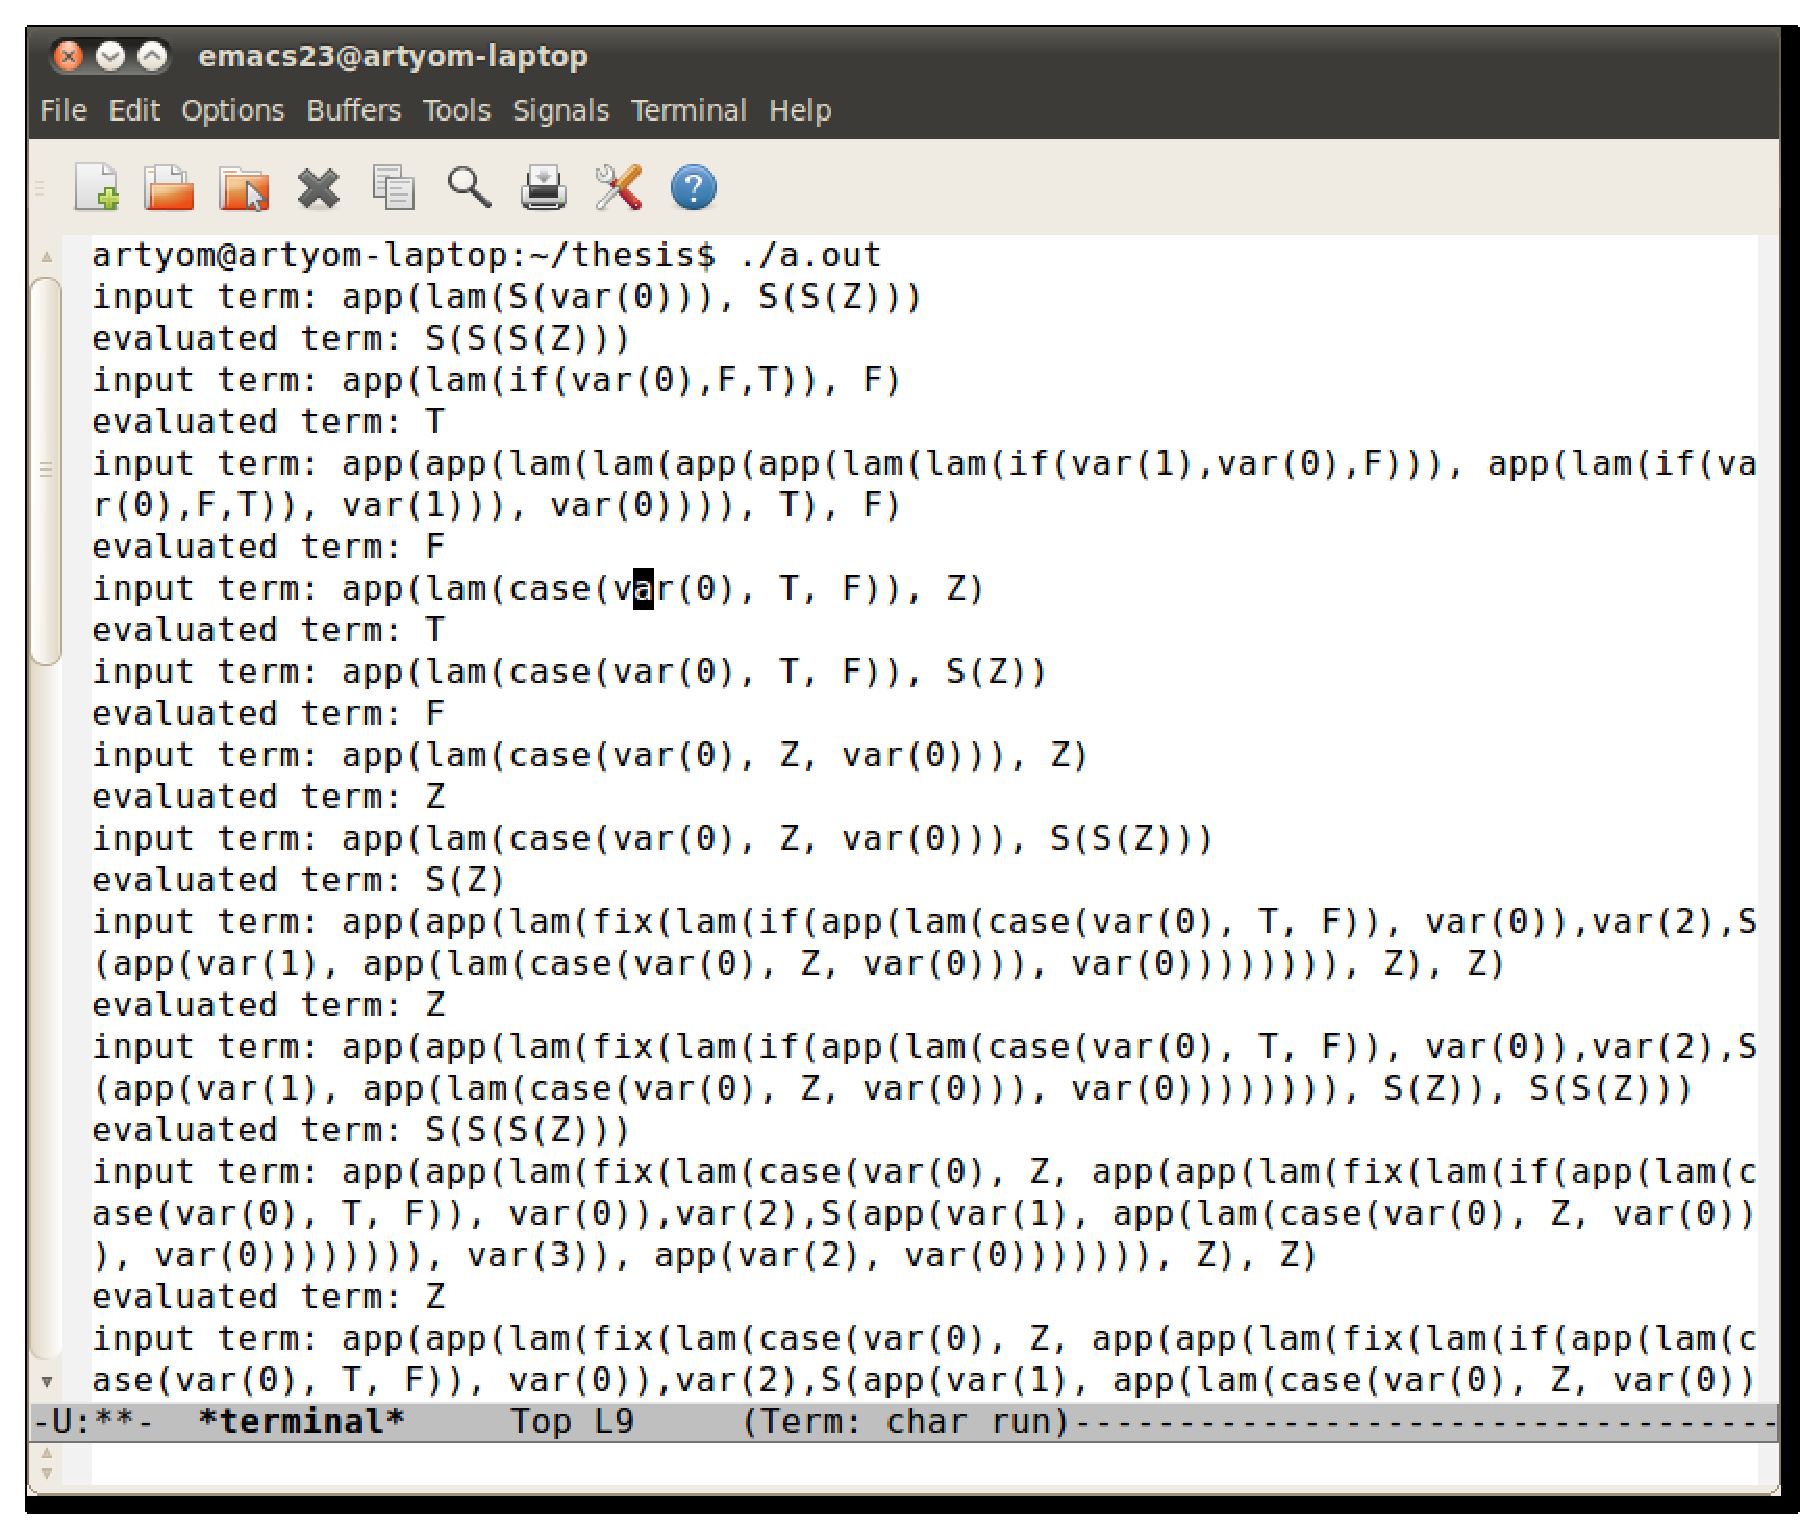
\includegraphics[width=0.8\linewidth]{term}}
  \end{figure}
}
\frame{
  \frametitle{Перспективы}
  \begin{itemize}
    \item Более выразительные системы типов
    \item Больше инвариантов
    \item Компиляция, управляемая типами
  \end{itemize}
}
\frame{
  \frametitle{Вопросы?}
}

\end{document}
